\chapter{Secure Device Identity}

A secure device identifier (DevID) is an identifier that is cryptographically bound to a device [\cite{DevIDSpec-IEEE}]. A device with DevID capability includes an Initial Device Identifier (IDevID) provided by the OEM. This IDevID must be stored in a way that protects it from modification. Since a TPM has capabilities to protect keys against compromise, it is an ideal choice for IDevID storage. Additionally, a device with DevID capability may support the creation of Locally Significant Device Identifiers (LDevIDs) by a device owner or network administrator (i.e., the Owner/Administrator). An LDevID cannot be transferred to a device with a different IDevID without knowledge of the private key used to produce the cryptographic binding.

When using a TPM key for secure device identity, there are restrictions on the attributes that it can have in order to enforce the best security practices; the key must have the \texttt{FixedTPM} and \texttt{Sign} attributes set and the \texttt{Decrypt} attribute not set. Furthermore the key may optionally have the \texttt{Restricted} attribute set. When the \texttt{Restricted} attribute is set, such a key is called an attestation key (AK). This DevID gets its special name due to its unique ability to be used as a parent node in a chain of certificates. The acronym AK is prefixed by the letter I or L denoting Initial or Locally Significant respectively. 



\begin{table}[h]
  \begin{center}
    \scriptsize 
    \sffamily
    \renewcommand{\arraystretch}{1.5}
    \begin{tabular}{ |c|c|c|c|c|c|c| }
      \hline
      Key & Type & \verb|FixedTPM| & \verb|Signing| & \verb|Decrypting| & \verb|Restricted| & Creator \\
      \hline
      \hline
      EK & Primary       & X &   & X & X & TPM Manufacturer \\
      \hline
      IAK & Primary      & X & X &   & X & OEM \\
      \hline
      IDevID & Primary   & X & X &   &   & OEM \\
      \hline
      LAK & Ordinary     & X & X &   & X & Owner/Admin \\
      \hline
      LDevID & Ordinary  & X & X &   &   & Owner/Admin \\
      \hline
    \end{tabular}
    \caption{Key Requirements and Recommendations}
    \label{fig:req_and_recs}
  \end{center}
\end{table}

The attribute requirements displayed in Table \ref{fig:req_and_recs} is modeled as a collection of functions. Each function takes a public key as input and returns a proposition.

\begin{figure}[h]
\begin{lstlisting}[language=Coq]
Definition endorsementKey (k : pubKey) : Prop :=
  match k with
  | Public _ Restricting NonSigning Decrypting => True
  | _ => False
  end.
\end{lstlisting}
\begin{lstlisting}[language=Coq]
Definition attestationKey (k : pubKey) : Prop :=
  match k with
  | Public _ Restricting Signing NonDecrypting => True
  | _ => False
  end.
\end{lstlisting}
\begin{lstlisting}[language=Coq]
Definition devidKey (k : pubKey) : Prop :=
  match k with
  | Public _ NonRestricting Signing NonDecrypting => True
  | _ => False
  end.
\end{lstlisting}
\caption{Model of Key Attribute Requirements}
\end{figure}

The issuers of device identity certificates are known as Certificate Authorities (CAs). CAs are further identified by the creator of the keys that they certify (i.e., the CA that issues certificates for IAKs and IDevIDs is known as the OEM's CA and the CA that issues certificates for LAKs and LDevIDs is known as the Owner/Administrator's CA). 
The OEM's CA must carefully verify the attributes and TPM residency of a key before signing a certificate due to the important security and identity implications provided by these certificates. 
All CAs should support a standard certificate transport protocol that provides confidentiality, integrity, and protection from replay attacks [\cite{DevIDSpec-TCG}]. These transport protocols are outside the scope of this paper. We will assume CAs to be following this recommendation precisely.


\section{Certificate Chain}

A chain of certificates can be used to verify a chain of trust to some trust anchor. The IAK certificate typically acts as this trust anchor.


\begin{figure}[h]
  \begin{centering}
  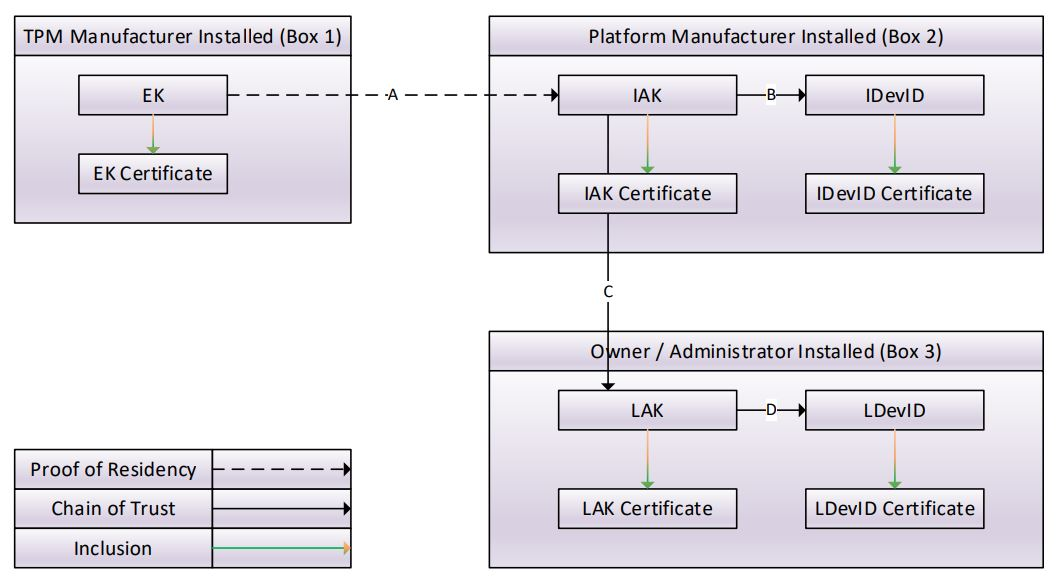
\includegraphics[width=.8\linewidth]{chap_3_figures/certificateRelationships.jpg}
  \par\end{centering}
  \caption{Key and Certificate Relationships [\cite{DevIDSpec-TCG}]}
  \label{fig:cert_rel}
\end{figure}

\begin{itemize}
  \item Box 1: The EK certificate is signed by the TPM Manufacturer's CA and binds the EK to a specific TPM.
  \item Line A: The IAK is verified by the OEM's CA to have the correct key properties and to be resident in the same TPM as the EK.
  \item Line B: The IDevID is verified by the OEM's CA to have the correct key properties and to be resident in the same TPM as the IAK.
  \item Box 2: The IAK certificate and IDevID certificate is signed by the OEM's CA and binds the IAK and IDevID to a specific device.
  \item Line C: The LAK is verified by the Owner/Administrator's CA to have the correct key properties and to be resident in the same TPM as the IAK.
  \item Line D: The LDevID is verified by the Owner/Administrator's CA to have the correct key properties and to be resident in the same TPM as the LAK.
  \item Box 3: The LAK certificate and LDevID certificate is signed by the Owner/Administrator's CA.
\end{itemize}

